\documentclass[../doc.tex]{subfiles}

\begin{document}
    Afin de faire l’UI, nous avons majoritairement utilisé l’outil de Unity Canvas. 
    Pour la direction artistique, compte tenu du thème de notre jeu portant sur les pirates, 
    nous avons décidé de nous inspirer du menu principal du jeu Sea Of Thieves. \newline
    
    \begin{figure}[hbt!]
        \centering
        \begin{subfigure}[t]{0.2\textwidth}
            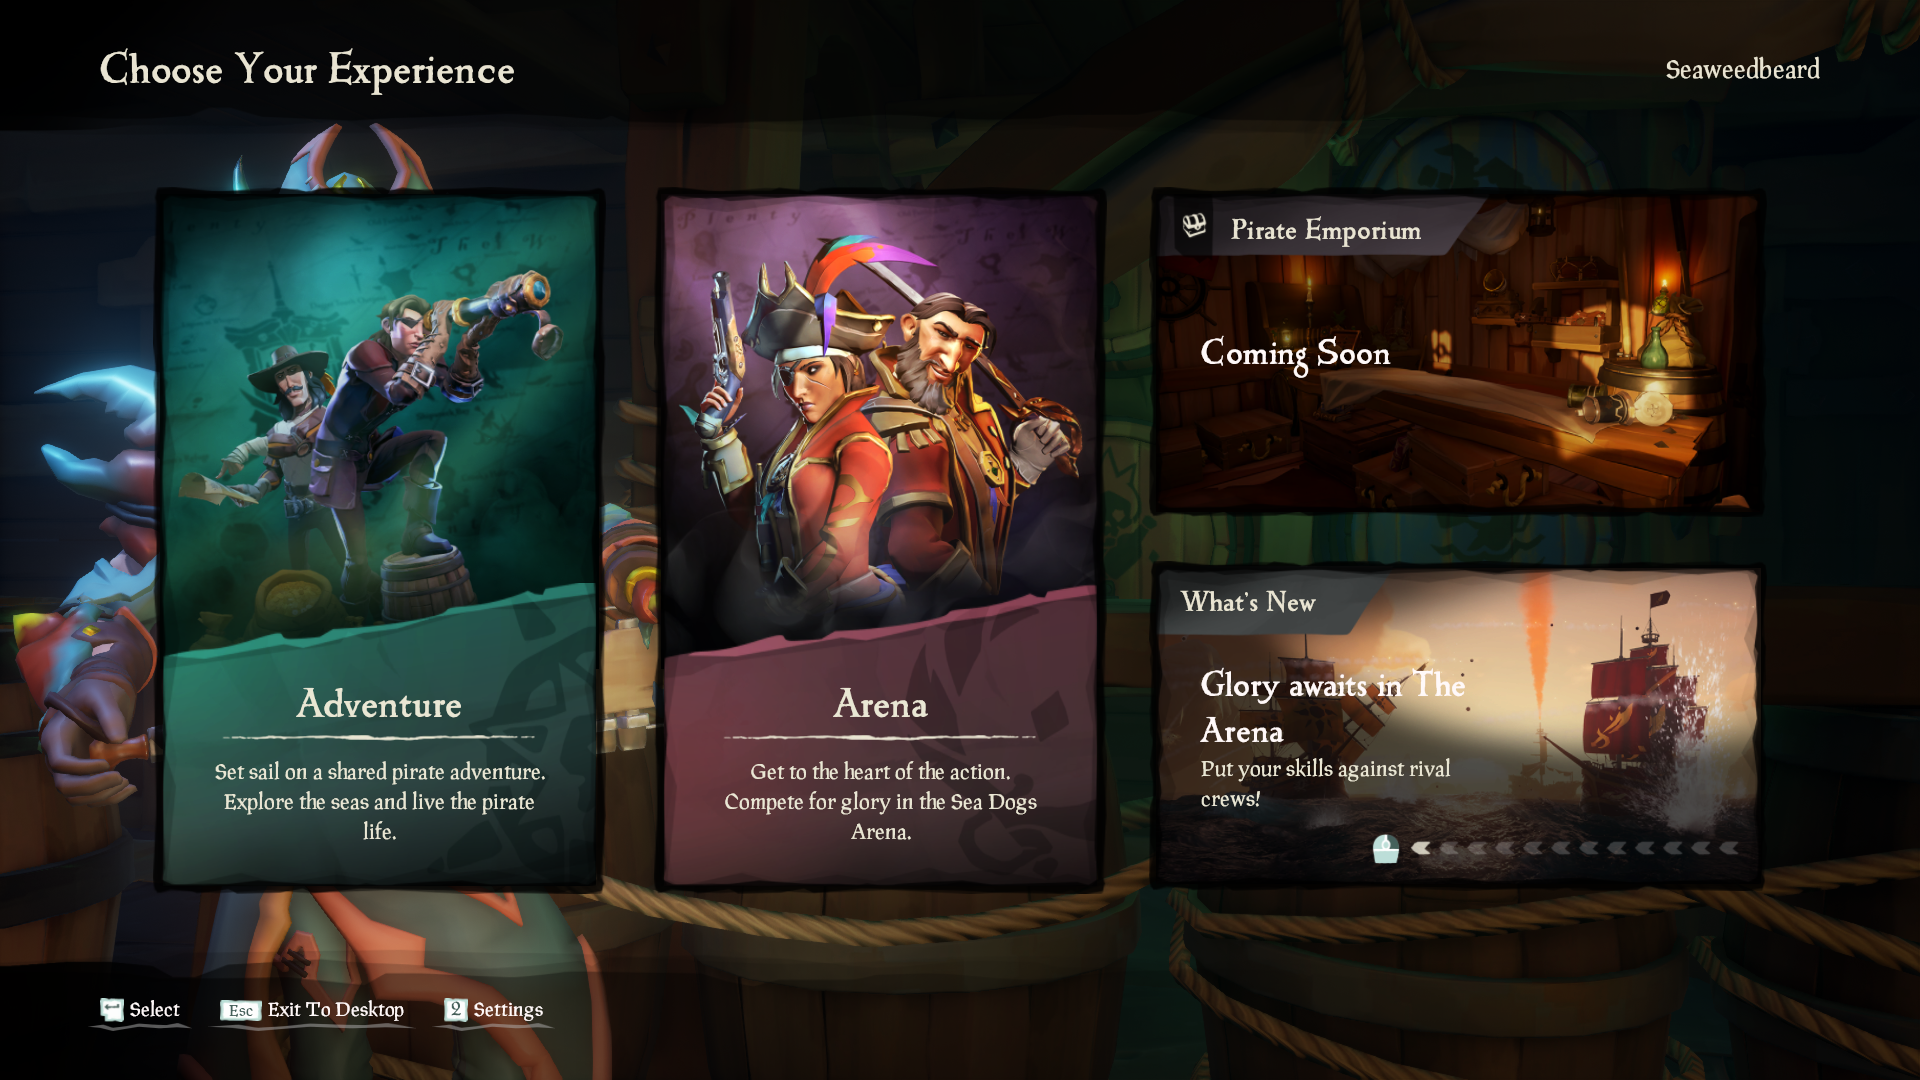
\includegraphics[scale=0.1]{sotmenu.png} 
            \caption{Menu de \texttt{Sea Of Thieves}}
        \end{subfigure}
        \hspace{125pt}
        \begin{subfigure}[t]{0.3\textwidth}
            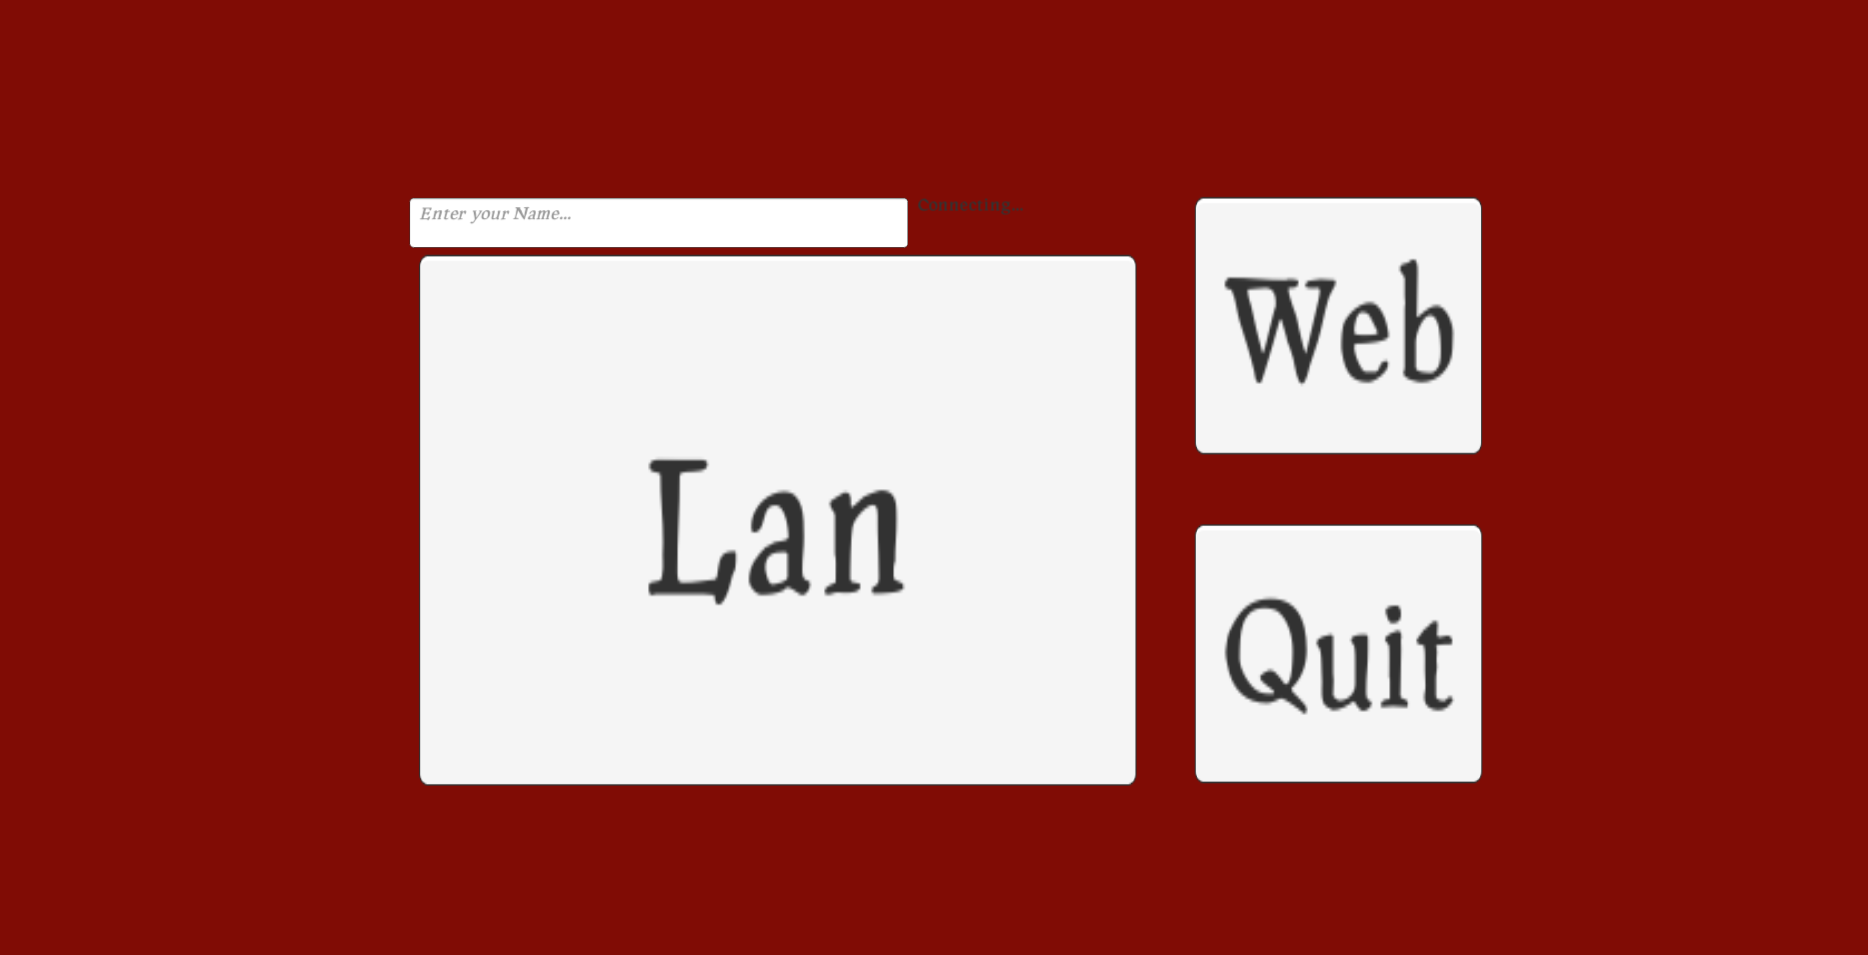
\includegraphics[scale=0.15]{menu.png}
            \caption{Menu du projet (Work in Progress)}
        \end{subfigure}
        \caption{Menus de Sea Of Thieves et de notre projet}
    \end{figure}
    
    Afin de rendre le menu plus vivant, 
    nous pourrions utiliser des animations sur les boutons ainsi que sur l’arrière-plan du menu.\newline 
    Notre menu intègrera 4 boutons et un champ. Le champ permettra au joueur d’entrer son nom dans le jeu. \newline
    Les 4 autres boutons serviront à :
    \begin{itemize}
        \item Se connecter à une partie
        \item Quitter le jeu
        \item Régler les paramètres du jeu
        \item Personnaliser son personnage
    \end{itemize}
\end{document}